\begin{frame}{Activity 1: put an inherited notebook in Git}
  \vfill
  \begin{columns}[c]
    \begin{column}{0.42\textwidth}
      \textbf{Start with the reactor notebook.}\\[0.8em]
      {\small Put its inputs, environment, changes, and results in Git so someone else can rerun and extend the work.}\\[1em]
      {\small The ZIP contains the notebook and parameter file. The handout walks through the steps.}\\[1em]
      {\small\href{https://raw.githubusercontent.com/dowlinglab/claude-for-researchers/main/resources/workshops/cstr/workshop1_notebook.zip}{\textbf{Download the notebook ZIP}}}
    \end{column}
    \begin{column}{0.54\textwidth}
      \centering
      \fbox{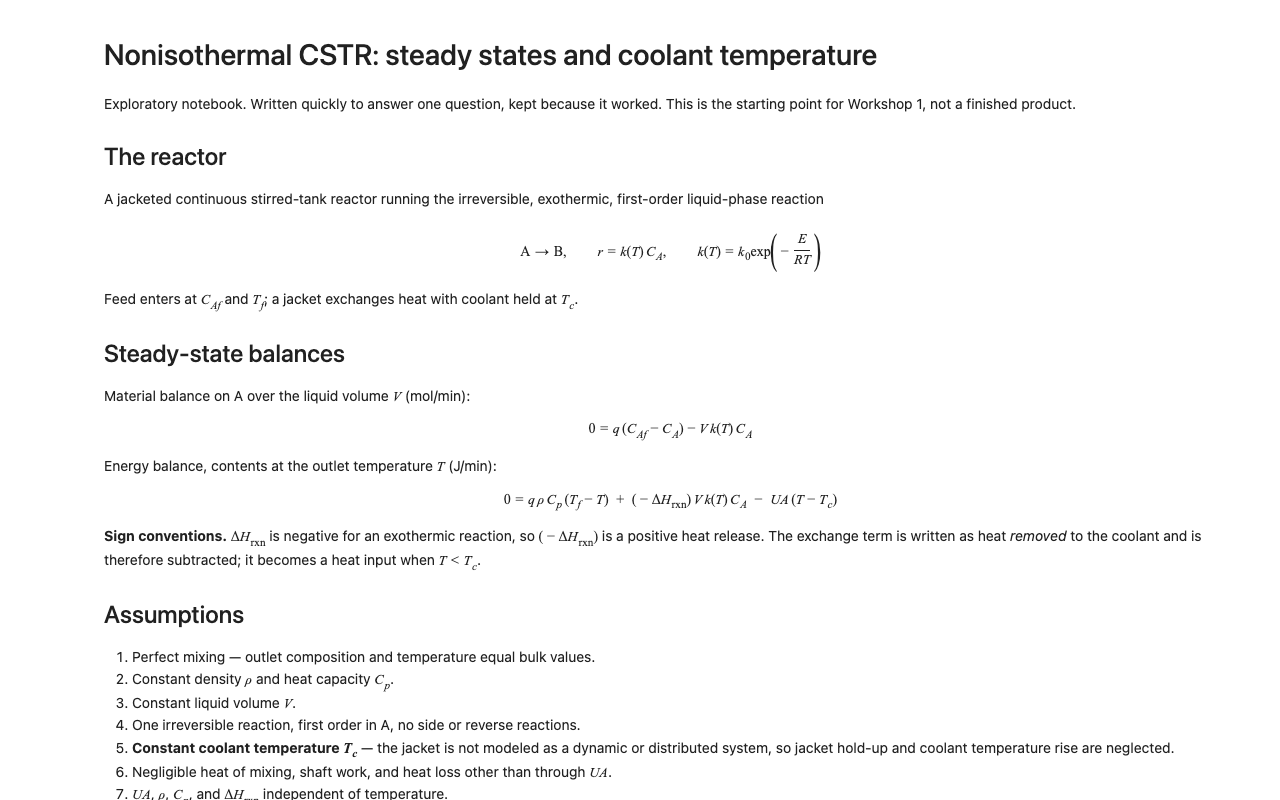
\includegraphics[width=0.94\linewidth]{figures/cstr_notebook_preview.png}}\\[0.3em]
      {\scriptsize The inherited CSTR notebook}
    \end{column}
  \end{columns}
  \vfill
  \ndlogonote{\scriptsize Hands-on: 45 minutes; regroup: 15 minutes}
\end{frame}

\begin{frame}{First, preserve what the inherited notebook does}
  \vfill
  \begin{enumerate}\setlength\itemsep{1em}
    \item \textbf{Create a private repository}
      \begin{itemize}\small
        \item Download the notebook handoff.
        \item Initialize Git.
        \item Commit the original files.
        \item Connect your private GitHub repository.
      \end{itemize}
    \item \textbf{Run and audit the notebook}
      \begin{itemize}\small
        \item Build the Conda environment.
        \item Run all notebook cells in a fresh kernel.
        \item Check the equations and input parameters.
        \item Check solver convergence and residuals.
        \item Check the saved CSV and figure.
        \item Commit the baseline before refactoring.
      \end{itemize}
  \end{enumerate}
  \vfill
  \ndlogonote{\scriptsize See the Part 1 handout for commands and full instructions}
\end{frame}

\begin{frame}{Then extract, test, and extend one question}
  \vfill
  \begin{enumerate}\setlength\itemsep{1em}
    \setcounter{enumi}{2}
    \item \textbf{Extract and verify functions}
      \begin{itemize}\small
        \item Extract the model equations into a Python file.
        \item Extract the steady-state solver.
        \item Extract the operating-condition sweep.
        \item Extract the plotting code.
        \item Add NumPy-style docstrings.
        \item Test against the saved baseline.
      \end{itemize}
    \item \textbf{Explore one new question}
      \begin{itemize}\small
        \item Choose one of the four extension questions.
        \item Save a runnable command.
        \item Save its result.
        \item Add a test.
        \item Write a short interpretation.
      \end{itemize}
  \end{enumerate}
  \vfill
\end{frame}
